%!TEX program = xelatex
\documentclass[a4paper,14pt]{extarticle}

% === Кодировка и язык ===
\usepackage{fontspec}
\setmainfont{Liberation Serif}
\setsansfont{Liberation Sans}
\setmonofont{Liberation Mono}

\usepackage{polyglossia}
\setdefaultlanguage{russian}
\setotherlanguage{english}

% === Геометрия страницы ===
\usepackage{geometry}
\geometry{
  a4paper,
  left=30mm, right=15mm,
  top=20mm, bottom=20mm
}

% === Межстрочный интервал ===
\usepackage{setspace}
\onehalfspacing

% === Оглавление и заголовки ===
\usepackage{titlesec}
\titleformat{\section}{\normalfont\large\bfseries}{\thesection.}{0.5em}{}
\titleformat{\subsection}{\normalfont\normalsize\bfseries}{\thesubsection.}{0.5em}{}

% === Колонтитулы ===
\usepackage{fancyhdr}
\setlength{\headheight}{17pt}
\pagestyle{fancy}
\fancyhf{}
\fancyhead[R]{\thepage}
\renewcommand{\headrulewidth}{0pt}

% === Работа с рисунками, таблицами, листингами ===
\usepackage{graphicx}
\usepackage{caption}
\usepackage{listings}
\usepackage{xcolor}
\usepackage{tabularx}
\usepackage{booktabs}
\usepackage{array}
\usepackage{longtable}
\usepackage{float}

% === Листинги кода ===
\lstdefinestyle{Cstyle}{
  language=C,
  basicstyle=\small\ttfamily,
  keywordstyle=\bfseries\color{black},
  commentstyle=\itshape\color{gray},
  stringstyle=\color{black},
  numbers=left,
  numberstyle=\tiny,
  stepnumber=1,
  numbersep=6pt,
  breaklines=true,
  frame=single,
  tabsize=2,
  showstringspaces=false,
  extendedchars=true,
  inputencoding=utf8
}

\lstdefinestyle{ASMstyle}{
  basicstyle=\small\ttfamily,
  numbers=none,
  breaklines=true,
  frame=single,
  tabsize=8,
  showstringspaces=false
}

\lstdefinestyle{PLIstyle}{
  basicstyle=\small\ttfamily,
  numbers=none,
  breaklines=true,
  frame=single,
  showstringspaces=false
}

% === Гиперссылки ===
\usepackage[hidelinks]{hyperref}

% === Прочее ===
\usepackage{enumitem}
\usepackage{amsmath}
\usepackage{indentfirst}
\setlength{\parindent}{1.25cm}

% === Подписи к рисункам ===
\captionsetup[figure]{name=Рис.,labelsep=period}
\captionsetup[table]{name=Таблица,labelsep=period}

\begin{document}

% ============================================================
% ТИТУЛЬНЫЙ ЛИСТ
% ============================================================
\thispagestyle{empty}
\begin{center}
  \textbf{Санкт-Петербургский политехнический университет}\\
  \textbf{Институт компьютерных наук и технологий}\\
  \textbf{Высшая школа программной инженерии}\\[3cm]

  {\Large\textbf{К У Р С О В А Я \quad Р А Б О Т А}}\\[1cm]
  {\large Разработка учебной системы программирования}\\[0.5cm]
  {\large Компилятор с ЯВУ}\\[2cm]

  Дисциплина: «Системы программирования»\\[1cm]
  Вариант~№~11\\[2cm]
\end{center}

\begin{flushright}
  \begin{tabular}{ll}
    Исполнители: & Студенты группы~5140904/50102\\
                 & Сырбу~Г.~В.\\
                 & Федерова~С.~К.\\[0.5cm]
    Руководитель: & Расторгуев~В.~Я.\\
  \end{tabular}
\end{flushright}

\vfill
\begin{center}
  Санкт-Петербург\\
  2026
\end{center}

\newpage

% ============================================================
% СОДЕРЖАНИЕ
% ============================================================
\tableofcontents
\newpage

% ============================================================
% РАЗДЕЛ 1. ЗАДАНИЕ НА КУРСОВУЮ РАБОТУ
% ============================================================
\section{Задание на курсовую работу}

Задание на курсовую работу дано в следующей общей формулировке:

\begin{quote}
«Необходимо выполнить доработку элементов макета учебной системы
программирования до уровня, позволяющего обрабатывать «новые» для макета
конструкции языка высокого уровня, примененные в соответствующем варианте».
\end{quote}

Общая формулировка персонализирована в варианте~№~11, приведённом на рис.~\ref{fig:variant}.

\begin{figure}[H]
\centering
\begin{lstlisting}[style=PLIstyle]
EX11: PROC OPTIONS ( MAIN );
DCL A BIN FIXED INIT ( 3 );
DCL B DEC FIXED INIT ( 3 );
DCL C BIN FIXED;
C = A = ( B * 5 );
END EX11;
\end{lstlisting}
\caption{Персональный вариант~№~11}
\label{fig:variant}
\end{figure}

По договорённости с преподавателем в персональный вариант были внесены
изменения, касающиеся использования скобок в арифметических выражениях:
вложенное выражение со скобками было разделено на два последовательных
оператора присваивания. В результате была сформулирована следующая входная
программа (рис.~\ref{fig:variant_mod}):

\begin{figure}[H]
\centering
\begin{lstlisting}[style=PLIstyle]
EX11: PROC OPTIONS ( MAIN );
DCL A BIN FIXED INIT ( 3 );
DCL B DEC FIXED INIT ( 3 );
DCL C BIN FIXED;
C = B * 5;
C = A = C;
END EX11;
\end{lstlisting}
\caption{Модифицированный персональный вариант~№~11 (согласованный с преподавателем)}
\label{fig:variant_mod}
\end{figure}

Схема функционирования макета учебной системы программирования, являющегося
согласно заданию на КР одним из элементов исходных данных, приведена на рис.~\ref{fig:arch}.

\begin{figure}[H]
\centering
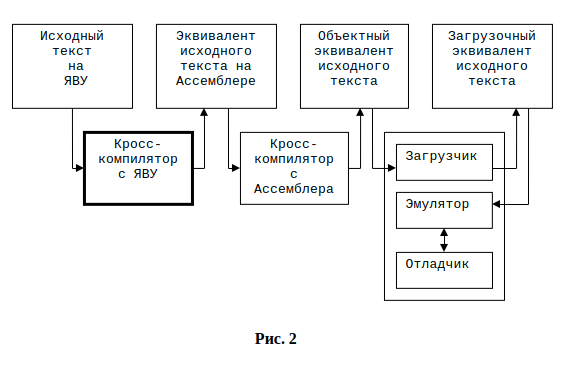
\includegraphics[width=\textwidth]{../источники/image.png}
\caption{Схема функционирования учебной системы программирования}
\label{fig:arch}
\end{figure}

Дополнительные требования к КР предполагают, что данная система программирования
работает на технологической ЭВМ (IBM PC) и является по существу кросс-системой для
объектной ЭВМ (IBM~370). В этой системе:
\begin{itemize}
  \item в качестве языка высокого уровня (ЯВУ) выбран язык, образованный из
        подмножества языковых конструкций PL/1; исходная программа готовится в виде
        текстового файла с расширением \texttt{*.pli};
  \item язык Ассемблера сформирован из языковых конструкций Ассемблера IBM~370;
        ассемблерный эквивалент исходной программы формируется в виде текстового
        файла с расширением \texttt{*.ass};
  \item объектный эквивалент исходной программы готовится в формате объектных файлов
        ОС IBM~370 и хранится в виде двоичного файла с расширением \texttt{*.tex};
  \item загрузочный эквивалент исходной программы представляет собой машинный код
        IBM~370, запоминаемый в области ОЗУ технологической ЭВМ, являющейся зоной
        загрузки для эмулятора объектной ЭВМ.
\end{itemize}

В данном отчёте документируются результаты модификации макетного компилятора с~ЯВУ
под персональный вариант~№~11.

\subsection*{Контрольный (демонстрационный) пример}

Контрольным примером, на который изначально настроен макет компилятора,
является программа \texttt{examppl.pli} (рис.~\ref{fig:demo}).

\begin{figure}[H]
\centering
\begin{lstlisting}[style=PLIstyle]
EXAMP: PROC OPTIONS ( MAIN );
DCL A BIN FIXED ( 31 ) INIT ( 11B  );
DCL B BIN FIXED ( 31 ) INIT ( 100B );
DCL C BIN FIXED ( 31 ) INIT ( 101B );
DCL D BIN FIXED ( 31 );
D = A + B - C;
END EXAMP;
\end{lstlisting}
\caption{Демонстрационный пример (\texttt{examppl.pli})}
\label{fig:demo}
\end{figure}

\subsection*{Отличия персонального варианта от демонстрационного примера}

Модифицированный персональный вариант~№~11 (рис.~\ref{fig:variant_mod})
приведён ниже:

\begin{lstlisting}[style=PLIstyle]
EX11: PROC OPTIONS ( MAIN );
DCL A BIN FIXED INIT ( 3 );
DCL B DEC FIXED INIT ( 3 );
DCL C BIN FIXED;
C = B * 5;
C = A = C;
END EX11;
\end{lstlisting}

При визуальном сравнении модифицированного персонального варианта~№~11
и демонстрационного примера (рис.~\ref{fig:demo}) выявлены следующие отличия:

\begin{enumerate}
  \item Переменные в персональном варианте объявляются без указания
        разрядности (без параметра в скобках), а инициализация задаётся
        десятичным целочисленным литералом (например, \texttt{3}) вместо
        двоичного (\texttt{11B}).

  \item В персональном варианте введена переменная \texttt{B} типа
        \texttt{DEC FIXED} (упакованный десятичный формат), тогда как в
        демонстрационном примере все переменные имеют тип \texttt{BIN FIXED}
        (двоичный формат с фиксированной точкой).

  \item В операторе \texttt{C = B * 5;} применяется операция умножения «\texttt{*}»
        упакованного десятичного операнда на десятичный целочисленный литерал,
        отсутствующая в демонстрационном примере.

  \item В операторе \texttt{C = A = C;} применяется знак логической операции
        «\texttt{=}» (сравнение) в правой части оператора присваивания,
        формирующий булево (логическое) значение; в модифицированной грамматике
        правая часть описывается нетерминалом \texttt{<AVL>}, а оператор в целом
        — нетерминалом \texttt{<OPL>} (см.\ раздел~3). Эта конструкция отсутствует
        в демонстрационном примере.
\end{enumerate}

% ============================================================
% РАЗДЕЛ 2. ПОСТАНОВКА ЗАДАЧИ
% ============================================================
\section{Постановка задачи модификации макета в части компилятора с ЯВУ}

Схема функционирования модифицированного макетного компилятора с~ЯВУ должна
соответствовать рис.~\ref{fig:compil_scheme}.

\begin{figure}[H]
\centering
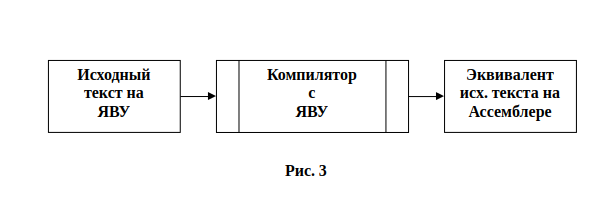
\includegraphics[width=\textwidth]{../источники/image2.png}
\caption{Схема функционирования модифицированного макетного компилятора с~ЯВУ}
\label{fig:compil_scheme}
\end{figure}

Функционал модифицированного макетного компилятора должен обеспечить компиляцию
исходного текста на ЯВУ (рис.~\ref{fig:variant_mod}) в эквивалент исходного текста на
Ассемблере, представленный на рис.~\ref{fig:etalon}.

\begin{figure}[H]
\centering
\begin{lstlisting}[style=ASMstyle]
  Метка       КОП       Операнды              Пояснения
EX11     START  0            Init rel addr=0
         BALR   @RBASE,0     Set @RBASE=cur PC
         USING  *,@RBASE     Use @RBASE for addr
         ZAP    @BUF(8),B(3) Copy pdec B->BUF
         MP     @BUF(8),@FIVE(1) Mul BUF by 5->BUF
         CVB    @R1,@BUF     pdec BUF ->int @R1
         STH    @R1,C        Store int ->C
         LH     @R2,A        Load A ->@R2
         CH     @R2,C        Compare @R2 with C
         BC     8,@TRUE      Branch if equal
         LA     @R3,0        Set @R3=0 (F)
         B      @SAVE        Jump to save
@TRUE    LA     @R3,1        Set @R3=1 (T)
@SAVE    STH    @R3,C        Store bool ->C
         BCR    15,@RVIX     Return to caller
A        DC     H'3'         Store halfword init
B        DC     PL3'3'       Store pdec init
C        DS     H            Reserve halfword
@FIVE    DC     PL1'5'       Store packed const
         DS     0F           Align next item
@BUF     DC     PL8'0'       Clear packed BUF
@RBASE   EQU    5            Set @RBASE=5
@R1      EQU    6            Set @R1=6
@R2      EQU    2            Set @R2=2
@R3      EQU    3            Set @R3=3
@RVIX    EQU    14           Set @RVIX=14
         END                 Program ends
\end{lstlisting}
\caption{Эталон ассемблерного эквивалента персонального варианта~№~11}
\label{fig:etalon}
\end{figure}

\subsection*{Согласованные функциональные ограничения}

По согласованию с преподавателем в модифицированном макетном компиляторе сохраняются
и уточняются следующие ограничения (согласованы с программой рис.~\ref{fig:variant_mod} и эталоном рис.~\ref{fig:etalon}):

\begin{enumerate}
  \item Компилятор не различает приоритеты арифметических операций в \texttt{<AVI>}: вычисление
        ведётся последовательно слева направо, без повышенного приоритета умножения относительно
        сложения и вычитания.

  \item Литерал-множитель в операции «\texttt{*}» (\texttt{AVI ZNK LID} в операторе \texttt{C = B * 5;})
        трактуется как десятичная однозначная константа в диапазоне $0$--$9$, что согласуется с
        упакованной однобайтовой константой в секции данных (см. \texttt{@FIVE} на рис.~\ref{fig:etalon}).

  \item Логическое выражение \texttt{<AVL>} в рассматриваемом варианте имеет вид сравнения
        \texttt{<AVI> ZNL <IPE>} (операнды — идентификаторы \texttt{BIN FIXED}, как в \texttt{C = A = C;}).
        Результат сравнения — булево значение \texttt{0}/\texttt{1} в формате halfword, записываемое в переменную
        слева от «\texttt{=}» в \texttt{<OPL>}.
\end{enumerate}

% ============================================================
% РАЗДЕЛ 3. МОДИФИКАЦИЯ БД КОМПИЛЯТОРА
% ============================================================
\section{Модификация состава и структуры БД макета компилятора с ЯВУ}

\subsection{Модификация БД лексического анализатора}

БД лексического анализатора определяется путём выделения подмножества терминальных
символов-разделителей термов языка. Функция лексического анализа в макете реализована
в подпрограмме \texttt{compress\_ISXTXT()}.

Для персонального варианта~№~11 разделителями термов являются терминальные символы
из множества:
\[
  \{\,\texttt{":"}\,,\, \texttt{"("}\,,\, \texttt{")"}\,,\, \texttt{";"}\,,\,
     \texttt{"+"}\,,\, \texttt{"-"}\,,\, \texttt{"="}\,,\, \texttt{"\_"}\,,\,
     \texttt{"*"}\,\}
\]

Модификация лексических настроек демонстрационного примера состоит в добавлении
символа умножения «\texttt{*}» в перечень разделителей термов. Данный символ в
оригинальном макете не входил в число обрабатываемых разделителей. Поскольку авторы
макета разместили перечень символов-разделителей непосредственно в теле подпрограммы
\texttt{compress\_ISXTXT()}, модификация выполнена в теле этой подпрограммы:

\begin{lstlisting}[style=Cstyle,caption={Фрагмент \texttt{compress\_ISXTXT()} с добавленным символом «\texttt{*}»},label=lst:lex]
void compress_ISXTXT()
{
  /* ... */
  if (
    ( ISXTXT[I1][I2] == '+' ||
      ISXTXT[I1][I2] == '-' ||
      ISXTXT[I1][I2] == '=' ||
      ISXTXT[I1][I2] == '(' ||
      ISXTXT[I1][I2] == ')' ||
      ISXTXT[I1][I2] == '*'   /* <- добавлен разделитель '*' */
    )
    && PREDSYM == ' '
  )
  { I3--; goto L1; }

  if ( ISXTXT[I1][I2] == ' ' &&
     ( PREDSYM == '+' || PREDSYM == '-' ||
       PREDSYM == '=' || PREDSYM == '*'   /* <- добавлен '*' */
     )
  )
  { goto L2; }
  /* ... */
}
\end{lstlisting}

\subsection{Модификация БД синтаксического анализатора}

Высокоуровневое определение модифицированного синтаксиса для персонального
варианта~№~11 приведено ниже; модификации по сравнению с грамматикой
демонстрационного примера выделены курсивом:

\begin{enumerate}
  \item $\langle\text{PRO}\rangle ::= \langle\text{OPR}\rangle\langle\text{TEL}\rangle\langle\text{OEN}\rangle$
  \item $\langle\text{OPR}\rangle ::= \langle\text{IPR}\rangle\texttt{:PROC\_OPTIONS(MAIN);}$
  \item $\langle\text{IPR}\rangle ::= \langle\text{IDE}\rangle$
  \item $\langle\text{IDE}\rangle ::= \langle\text{BUK}\rangle \mid \langle\text{IDE}\rangle\langle\text{BUK}\rangle \mid \langle\text{IDE}\rangle\langle\text{CIF}\rangle$
  \item $\langle\text{BUK}\rangle ::= \texttt{A} \mid \texttt{B} \mid \texttt{C} \mid \texttt{D} \mid \texttt{E} \mid \texttt{M} \mid \texttt{P} \mid \texttt{X}$
  \item $\langle\text{CIF}\rangle ::= \texttt{0} \mid \texttt{1} \mid \texttt{2} \mid \texttt{3} \mid \texttt{4} \mid \texttt{5} \mid \texttt{6} \mid \texttt{7} \mid \texttt{8} \mid \texttt{9}$
  \item $\langle\text{TEL}\rangle ::= \langle\text{ODC}\rangle \mid \langle\text{TEL}\rangle\langle\text{ODC}\rangle \mid \langle\text{TEL}\rangle\langle\text{OPA}\rangle \mid \langle\text{TEL}\rangle\langle\text{OPL}\rangle$
  \item $\langle\text{ODC}\rangle ::= \texttt{DCL\_}\langle\text{IPE}\rangle\texttt{\_BIN\_FIXED(}\langle\text{RZR}\rangle\texttt{);}$\\
        $\mid\; \texttt{DCL\_}\langle\text{IPE}\rangle\texttt{\_BIN\_FIXED(}\langle\text{RZR}\rangle\texttt{)INIT(}\langle\text{LIT}\rangle\texttt{);}$\\
        \textit{$\mid\; \texttt{DCL\_}\langle\text{IPE}\rangle\texttt{\_BIN\_FIXED;}$}\\
        \textit{$\mid\; \texttt{DCL\_}\langle\text{IPE}\rangle\texttt{\_BIN\_FIXED\_INIT(}\langle\text{LID}\rangle\texttt{);}$}\\
        \textit{$\mid\; \texttt{DCL\_}\langle\text{IPE}\rangle\texttt{\_DEC\_FIXED\_INIT(}\langle\text{LID}\rangle\texttt{);}$}
  \item $\langle\text{IPE}\rangle ::= \langle\text{IDE}\rangle$
  \item $\langle\text{RZR}\rangle ::= \langle\text{CIF}\rangle \mid \langle\text{RZR}\rangle\langle\text{CIF}\rangle$
  \item $\langle\text{LIT}\rangle ::= \langle\text{MAN}\rangle\texttt{B}$
  \item $\langle\text{MAN}\rangle ::= \texttt{1} \mid \langle\text{MAN}\rangle\texttt{0} \mid \langle\text{MAN}\rangle\texttt{1}$
  \item \textit{$\langle\text{LID}\rangle ::= \langle\text{CIF}\rangle \mid \langle\text{LID}\rangle\langle\text{CIF}\rangle$}
  \item $\langle\text{OPA}\rangle ::= \langle\text{IPE}\rangle\texttt{=}\langle\text{AVI}\rangle\texttt{;}$
  \item $\langle\text{AVI}\rangle ::= \langle\text{LIT}\rangle \mid \langle\text{LID}\rangle \mid \langle\text{IPE}\rangle$\\
        $\mid\; \langle\text{AVI}\rangle\langle\text{ZNK}\rangle\langle\text{LIT}\rangle
        \mid \langle\text{AVI}\rangle\langle\text{ZNK}\rangle\langle\text{LID}\rangle
        \mid \langle\text{AVI}\rangle\langle\text{ZNK}\rangle\langle\text{IPE}\rangle$
  \item $\langle\text{AVL}\rangle ::= \langle\text{AVI}\rangle\langle\text{ZNL}\rangle\langle\text{LIT}\rangle
        \mid \langle\text{AVI}\rangle\langle\text{ZNL}\rangle\langle\text{LID}\rangle
        \mid \langle\text{AVI}\rangle\langle\text{ZNL}\rangle\langle\text{IPE}\rangle$
  \item $\langle\text{OPL}\rangle ::= \langle\text{IPE}\rangle\texttt{=}\langle\text{AVL}\rangle\texttt{;}$
  \item $\langle\text{ZNK}\rangle ::= \texttt{+} \mid \texttt{-}$ \textit{$\mid\; \texttt{*}$}
  \item \textit{$\langle\text{ZNL}\rangle ::= \texttt{=}$}
  \item $\langle\text{OEN}\rangle ::= \texttt{END\_}\langle\text{IPR}\rangle$
\end{enumerate}

Пояснения к метасимволам:
\begin{itemize}
  \item \texttt{<} и \texttt{>} — ограничители нетерминального символа;
  \item \texttt{::=} — «равно по определению»;
  \item \texttt{|} — альтернативное определение («или»);
  \item \texttt{\_} — терминальный символ «пробел».
\end{itemize}

Перечень нетерминальных символов приведён в таблице~\ref{tab:nonterm}.

\begin{table}[H]
\centering
\caption{Нетерминальные символы грамматики}
\label{tab:nonterm}
\begin{tabularx}{\textwidth}{|l|X|}
  \hline
  \textbf{Нетерминал} & \textbf{Смысл} \\
  \hline
  \texttt{<PRO>} & программа \\
  \texttt{<OPR>} & оператор пролога программы \\
  \texttt{<IPR>} & имя программы \\
  \texttt{<IDE>} & идентификатор \\
  \texttt{<BUK>} & буква \\
  \texttt{<CIF>} & цифра \\
  \texttt{<TEL>} & тело программы \\
  \texttt{<ODC>} & оператор объявления переменных (DCL) \\
  \texttt{<IPE>} & имя переменной \\
  \texttt{<RZR>} & разрядность \\
  \texttt{<LIT>} & двоичный литерал \\
  \texttt{<MAN>} & мантисса литерала \\
  \texttt{<LID>} & десятичный целочисленный литерал \\
  \texttt{<OPA>} & оператор присваивания (арифметическое выражение) \\
  \texttt{<OPL>} & оператор присваивания (логическое выражение) \\
  \texttt{<AVI>} & арифметическое выражение \\
  \texttt{<AVL>} & логическое выражение \\
  \texttt{<ZNK>} & знак арифметической операции \\
  \texttt{<ZNL>} & знак логической операции \\
  \texttt{<OEN>} & оператор эпилога программы (END) \\
  \hline
\end{tabularx}
\end{table}

По сравнению с грамматикой демонстрационного примера модифицированы правила:
\begin{itemize}
  \item \textbf{Правило~7 (\texttt{<TEL>}):} добавлена альтернатива
        \texttt{<TEL><OPL>} для операторов присваивания с логическим выражением
        в правой части;
  \item \textbf{Правило~8 (\texttt{<ODC>}):} в подмножестве, используемом
        демонстрационным примером и модифицированным персональным вариантом~№~11,
        сохранены объявления \texttt{BIN FIXED} с разрядностью и двоичной
        инициализацией (демонстрационный пример), а также объявления без
        разрядности и с инициализацией десятичным литералом \texttt{<LID>}
        (персональный вариант); альтернативы \texttt{DEC FIXED} с указанием
        разрядности и без инициализации исключены как не встречающиеся в
        указанных программах;
  \item \textbf{Правило~13 (\texttt{<LID>}):} введён новый нетерминал
        для десятичного целочисленного литерала (аналог \texttt{<LIT>} для
        десятичной записи), используемый при объявлении переменных без
        разрядности и в арифметических выражениях;
  \item \textbf{Правило~15 (\texttt{<AVI>}):} добавлена возможность применения
        нетерминала~\texttt{<LID>} как самостоятельного операнда; логические
        комбинации со знаком \texttt{<ZNL>} вынесены в отдельное правило
        \texttt{<AVL>} (правило~16);
  \item \textbf{Правило~16 (\texttt{<AVL>}):} введён нетерминал логического
        выражения — сравнение двух операндов посредством \texttt{<ZNL>}, где
        левый операнд задаётся \texttt{<AVI>};
  \item \textbf{Правило~17 (\texttt{<OPL>}):} введён оператор присваивания
        с правой частью \texttt{<AVL>} (аналог \texttt{<OPA>} для логических
        выражений);
  \item \textbf{Правило~18 (\texttt{<ZNK>}):} к знакам «\texttt{+}» и
        «\texttt{-}» добавлен знак «\texttt{*}» (умножение);
  \item \textbf{Правило~19 (\texttt{<ZNL>}):} введён нетерминал для знака
        логической операции «\texttt{=}» (сравнение), не входящий в
        \texttt{<ZNK>}; различение арифметических и логических знаков
        производится по контексту их использования в грамматике.
\end{itemize}

В состав нетерминальных символов после модификации добавлены нетерминалы
\texttt{<LID>} (десятичный целочисленный литерал), \texttt{<ZNL>} (знак
логической операции), \texttt{<AVL>} (логическое выражение) и \texttt{<OPL>}
(оператор присваивания с логическим выражением).

\subsubsection*{Модификация таблицы синтаксических правил \texttt{SINT[]}}

Таблица \texttt{SINT[]} реализует двунаправленный список с альтернативными
ветвлениями, в котором каждая запись описывает один шаг распознавания (форма
распознавания — от правой части к нетерминалу). В ходе модификации:

\begin{itemize}
  \item размер таблицы увеличен; добавлены записи, описывающие новые
        ветки грамматики: альтернативы объявлений \texttt{ODC} без разрядности
        с использованием нетерминала \texttt{<LID>}, ветка распознавания
        нетерминала \texttt{<ZNL>} для знака логической операции «\texttt{=}»,
        ветки для \texttt{<LID>} в качестве операнда выражения \texttt{<AVI>},
        а также ветки для \texttt{<AVL>} и \texttt{<OPL>};
  \item в существующих записях изменены поля альтернативы \texttt{ALT}
        для обеспечения перехода к новым веткам грамматики.
\end{itemize}

\subsubsection*{Дополнение таблицы \texttt{SINT[]}: ветви \texttt{LID}, \texttt{ZNL}, \texttt{AVL}, \texttt{OPL}}

Объём таблицы \texttt{SINT[]} увеличивается (условно: \texttt{\#define NSINT~260}); после существующих записей добавляются цепочки,
соответствующие правилам из разд.~3. Фрагмент новых записей приведён в листинге~\ref{lst:sint_new4} (номера записей и поля \texttt{ALT}
согласуются с конкретной нумерацией в исходном \texttt{komppl.c}; ниже — типичная структура ветвлений).

\begin{figure}[H]
\begin{lstlisting}[style=Cstyle,caption={Фрагмент новых записей \texttt{SINT[]} (ветви \texttt{LID}, \texttt{ZNL}, \texttt{AVL}, \texttt{OPL})},label=lst:sint_new4]
 /* BIN_FIXED без разрядности: ... FIXED ; */
 {/*.  232     .*/   233 ,   187 , "D  " ,    0 },
 /* ... распознавание BIN / DEC, INIT(LID) для персонального варианта ... */
 /* LID как терминальная цепочка (цифры) для INIT и AVI */
 {/*.  240     .*/   241 ,     0 , "LID" ,    0 },
 {/*.  241     .*/   242 ,   240 , "CIF" ,    0 },
 /* OPL:  IPE = AVL ; */
 {/*.  245     .*/   246 ,   165 , "OPL" ,    0 },
 {/*.  246     .*/   247 ,   245 , "IPE" ,    0 },
 {/*.  247     .*/   248 ,   246 , "=  " ,    0 },
 {/*.  248     .*/   249 ,   247 , "AVL" ,    0 },
 {/*.  249     .*/   250 ,   248 , ";  " ,    0 },
 /* AVL:  AVI ZNL ( IPE | LIT | LID ) — здесь ZNL отделён от ZNK */
 {/*.  251     .*/   252 ,   165 , "AVI" ,    0 },
 {/*.  252     .*/   253 ,   251 , "ZNL" ,    0 },
 {/*.  253     .*/     0 ,   252 , "*  " ,    0 },
 /* ZNL: знак '=' (логическое сравнение), не путать с присваиванием */
 {/*.  254     .*/   255 ,     0 , "=  " ,    0 },
 {/*.  255     .*/     0 ,   254 , "ZNL" ,    0 }
\end{lstlisting}
\end{figure}

Кроме добавления записей, в ряде существующих строк изменяется поле \texttt{ALT}: например, у ветки распознавания
оператора присваивания добавляется альтернатива перехода к цепочке \texttt{OPL} (если по контексту ожидается логическое выражение),
а у строки, где ранее символ «\texttt{=}» относился только к устаревшему объединённому знаку операции, задаётся переход к цепочке \texttt{ZNL}.

\subsubsection*{Модификация таблицы входов \texttt{VXOD[]} и матрицы \texttt{TPR[][]}}

В таблице \texttt{VXOD[]} регистрируются начальные символы цепочек распознавания нетерминалов. Для десятичного литерала \texttt{<LID>}
добавляется строка с лексическим образом числового терма и полем \texttt{VX}, указывающим на первую запись цепочки \texttt{LID}
(листинг~\ref{lst:vxod4}). Для знака «\texttt{=}» поле \texttt{VX} настраивается на распознавание \texttt{<ZNL>} (логическое сравнение)
в контексте правила \texttt{<AVL>}; различение присваивания и сравнения обеспечивается за счёт структуры \texttt{SINT[]} и порядка
свёрток при разборе \texttt{<OPA>} / \texttt{<OPL>} (см. листинг~\ref{lst:sint_new4}).

\begin{lstlisting}[style=Cstyle,caption={Фрагмент изменений в \texttt{VXOD[]}},label=lst:vxod4]
  /* Цепочка LID (десятичный литерал) */
  {/*.  NN      .*/   "LID" , 240 , 'N' },
  /* Символ '=' — переход к ZNL (не к арифметическому ZNK) */
  {/*.  50      .*/   "=  " , 254 , 'T' },
\end{lstlisting}

В матрице предшествования \texttt{TPR[][]} добавляются строки/столбцы, соответствующие новым нетерминалам \texttt{LID}, \texttt{ZNL},
\texttt{AVL}, \texttt{OPL}: устанавливаются отношения предшествования между символами «\texttt{=}», «\texttt{;}» и новыми
нетерминалами так, чтобы сохранить детерминированность разбора для персонального варианта (линейная форма \texttt{AVI}, одно сравнение
в \texttt{AVL}).

% ============================================================
% РАЗДЕЛ 4. МОДИФИКАЦИЯ АЛГОРИТМА
% ============================================================
\section{Модификация алгоритма макета компилятора с ЯВУ}

Модификация алгоритма второго прохода связана с появлением новых нетерминалов \texttt{<LID>}, \texttt{<ZNL>},
\texttt{<AVL>}, \texttt{<OPL>} (табл.~\ref{tab:nonterm}): требуется разделить обработку арифметики (\texttt{AVI2()})
и логического сравнения (\texttt{AVL2()}), а также ввести \texttt{OPL2()} для присваивания результата \texttt{<AVL>}.
Подпрограмма \texttt{ODC1()} расширяется для объявлений без разрядности и инициализации десятичным \texttt{<LID>}.

Анализ изменений в правилах грамматики определяет перечень подпрограмм, подлежащих модификации:

\begin{itemize}
  \item \textbf{\texttt{ODC1()}} — добавлена обработка альтернатив \texttt{BIN FIXED;} и \texttt{BIN FIXED INIT ( LID )},
        \texttt{DEC FIXED INIT ( LID )} с записью инициализатора в \texttt{SYM[ ].INIT} как десятичной строки;
  \item \textbf{\texttt{AVI2()}} — обрабатывает только знаки \texttt{<ZNK>} (\texttt{+}, \texttt{-}, \texttt{*}) и операнды
        \texttt{LIT}, \texttt{LID}, \texttt{IPE}; ветвь сравнения «\texttt{=}» перенесена в \texttt{AVL2()};
  \item \textbf{\texttt{AVL2()}} — \textit{новая} подпрограмма: после вычисления левого \texttt{<AVI>} генерирует цепочку
        \texttt{LH}/\texttt{CH}/\texttt{BC}/\texttt{LA}/\texttt{B}/\texttt{STH} для булева результата (как на рис.~\ref{fig:etalon});
  \item \textbf{\texttt{OPA2()}} — присваивание результата арифметического \texttt{<AVI>} (без изменения логики сравнения);
  \item \textbf{\texttt{OPL2()}} — \textit{новая} подпрограмма: оформляет присваивание результата \texttt{AVL2()} в переменную
        типа \texttt{BIN FIXED} (аналог \texttt{OPA2()} для \texttt{<OPL>});
  \item \textbf{\texttt{OEN2()}} — генерация \texttt{DC H'...'} из десятичного \texttt{INIT} и \texttt{PL...'} для \texttt{DEC FIXED};
  \item \textbf{\texttt{OPR2()}} — без принципиальных изменений относительно эталона (пролог \texttt{START}/\texttt{BALR}/\texttt{USING}).
\end{itemize}

Дополнительно используются вспомогательные механизмы из макета:
\begin{itemize}
  \item глобальные переменные \texttt{RESULT\_REG}, \texttt{PENDING\_LABEL}, массив \texttt{EXTRA[]} для констант умножения;
  \item подпрограммы \texttt{SETCOMM()} и \texttt{const\_label()} для комментариев и имён упакованных констант.
\end{itemize}

\subsection{Новые глобальные переменные}

Структура глобальных переменных соответствует принятой в макете схеме передачи регистра результата и отложенной метки
для ветвления сравнения (листинг~\ref{lst:globals4}).

\begin{lstlisting}[style=Cstyle,caption={Глобальные переменные (фрагмент)},label=lst:globals4]
char RESULT_REG[9]  = "@R2";
char PENDING_LABEL[9] = "";
struct {
    char name[9];
    char type;
    int  size;
    char value[10];
} EXTRA[20];
int NEXTRA = 0;
\end{lstlisting}

\subsection{Вспомогательные подпрограммы \texttt{SETCOMM()} и \texttt{const\_label()}}

Назначение подпрограмм — как в базовом макете: \texttt{SETCOMM()} записывает пояснение в поле комментария ассемблерной карточки;
\texttt{const\_label()} формирует имя упакованной константы (\texttt{@FIVE} для множителя \texttt{5}).

\subsection{Модификация подпрограммы \texttt{ODC1()}}

В \texttt{ODC1()} добавляется разбор объявлений без скобок с разрядностью: ключевые слова \texttt{BIN FIXED} / \texttt{DEC FIXED},
признак \texttt{INIT}, в скобках — цепочка, распознанная как \texttt{<LID>}. Для \texttt{DEC FIXED} задаётся тип \texttt{'D'} и
длина упакованного поля по соглашению макета (например, \texttt{PL3} для значений из примера); для \texttt{BIN FIXED} без инициализации
поле \texttt{INIT} очищается, для инициализации десятичным литералом строка цифр копируется в \texttt{SYM[ ].INIT} для последующего
\texttt{VALUE()} на втором проходе.

\subsection{Модификация подпрограммы \texttt{AVI2()}}

Подпрограмма генерирует код только для \texttt{<AVI>}: загрузка \texttt{LIT}/\texttt{LID}/\texttt{IPE}, операции \texttt{+}, \texttt{-}, \texttt{*}
с последовательным обновлением \texttt{RESULT\_REG}. Для \texttt{DEC FIXED} перед умножением на \texttt{LID} сохраняется схема
\texttt{ZAP}/\texttt{MP}/\texttt{CVB} из эталона. Ветка с символом «\texttt{=}» из \texttt{<ZNK>} \textbf{не} обрабатывается в \texttt{AVI2()}.

\subsection{Подпрограмма \texttt{AVL2()}}

Новая подпрограмма вызывается при свёртке к \texttt{<AVL>}: к моменту обработки левое подвыражение \texttt{<AVI>} уже сведено к значению
в регистре \texttt{@R2} (для \texttt{BIN FIXED}). Далее генерируются инструкции \texttt{CH}, \texttt{BC}, ветви \texttt{LA} для \texttt{0}/\texttt{1},
переход \texttt{B @SAVE}, метка \texttt{@TRUE}, установка \texttt{PENDING\_LABEL} для последующего \texttt{STH} в \texttt{OPL2()} —
в соответствии с рис.~\ref{fig:etalon}.

\subsection{Модификация подпрограммы \texttt{OPA2()}}

Для \texttt{<OPA>} сохраняется запись результата \texttt{<AVI>} (например, \texttt{STH @R1,C} после умножения). Обработка булева результата
перенесена в \texttt{OPL2()}.

\subsection{Подпрограмма \texttt{OPL2()}}

По аналогии с \texttt{OPA2()}: размещение результата сравнения из \texttt{RESULT\_REG} (\texttt{@R3}) в полуслово целевой переменной,
навешивание отложенной метки \texttt{PENDING\_LABEL} (\texttt{@SAVE}) на карточку \texttt{STH}.

\subsection{Модификация подпрограммы \texttt{OEN2()}}

Эпилог формирует секцию данных: \texttt{DC H'd'} для \texttt{BIN FIXED} с десятичным инициализатором (\texttt{H'3'} для \texttt{3}),
\texttt{DC PL3'3'} для \texttt{DEC FIXED}, \texttt{DS H} для неинициализированной \texttt{C}, константы \texttt{EXTRA[]}, буфер \texttt{@BUF},
директивы \texttt{EQU}, \texttt{END} — в соответствии с рис.~\ref{fig:etalon}.

\subsection{Модификация подпрограммы \texttt{OPR2()}}

Генерация пролога (\texttt{START}, \texttt{BALR}, \texttt{USING}) без изменения идеологии относительно эталона.

% ============================================================
% РАЗДЕЛ 5. РЕЗУЛЬТАТЫ ЭКСПЕРИМЕНТАЛЬНОЙ ПРОВЕРКИ
% ============================================================
\section{Результаты экспериментальной проверки модифицированного компилятора с ЯВУ}

Работоспособность модифицированного макетного компилятора с~ЯВУ может быть подтверждена испытательным прогоном в среде ОС~Linux
(сборка \texttt{gcc~-m32}, см. \texttt{Makefile} в каталоге \texttt{lab-step-2}).

Команды сборки и запуска (из каталога \texttt{lab-step-2}):

\begin{lstlisting}[style=ASMstyle,caption={Сборка и запуск компилятора},label=lst:build4]
make
./build/komppl.exe input/ex11.pli
\end{lstlisting}

В качестве эталона выходного текста используется листинг на рис.~\ref{fig:etalon}; полученный файл \texttt{output/ex11.ass} (или
\texttt{ex11.ass} в рабочем каталоге по настройке макета) сопоставляется с эталоном построчно.

\begin{figure}[H]
\begin{lstlisting}[style=ASMstyle,caption={Ожидаемый фрагмент ассемблерного вывода (совпадение с рис.~\ref{fig:etalon})},label=lst:result_asm4]
EX11     START 0            Init rel addr=0
         BALR  @RBASE,0     Set @RBASE=cur PC
         USING *,@RBASE     Use @RBASE for addr
         ZAP   @BUF(8),B(3) Copy pdec B->BUF
         MP    @BUF(8),@FIVE(1) Mul BUF by 5 ->BUF
         CVB   @R1,@BUF     pdec BUF ->int @R1
         STH   @R1,C        Store int ->C
         LH    @R2,A        Load A ->@R2
         CH    @R2,C        Compare @R2 with C
         BC    8,@TRUE      Branch if equal
         LA    @R3,0        Set @R3=0 (F)
         B     @SAVE        Jump to save
@TRUE    LA    @R3,1        Set @R3=1 (T)
@SAVE    STH   @R3,C        Store bool ->C
         BCR   15,@RVIX     Return to caller
A        DC    H'3'         Store halfword init
B        DC    PL3'3'       Store pdec init
C        DS    H            Reserve halfword
@FIVE    DC    PL1'5'       Store packed const
         DS    0F           Align next item
@BUF     DC    PL8'0'       Clear packed BUF
@RBASE   EQU   5            Set @RBASE=5
@R1      EQU   6            Set @R1=6
@R2      EQU   2            Set @R2=2
@R3      EQU   3            Set @R3=3
@RVIX    EQU   14           Set @RVIX=14
         END                Program ends
\end{lstlisting}
\end{figure}

\subsection*{Пояснения к сгенерированному тексту}

\textbf{Семантика исходной программы} (рис.~\ref{fig:variant_mod}): \texttt{A = 3}, \texttt{B = 3} (упаковано);
\texttt{C = B * 5} даёт \texttt{C = 15}; \texttt{C = A = C} — сравнение \texttt{A} и \texttt{C}, результат «ложь», \texttt{C := 0}.

\textbf{Оператор \texttt{C = B * 5;}} формируется цепочкой \texttt{ZAP}/\texttt{MP}/\texttt{CVB}/\texttt{STH} (\texttt{AVI2()}).

\textbf{Оператор \texttt{C = A = C;}} соответствует \texttt{<OPL>}: \texttt{AVL2()} строит сравнение и булев результат,
\texttt{OPL2()} записывает его в \texttt{C}.

% ============================================================
% РАЗДЕЛ 6. ВЫВОДЫ
% ============================================================
\section{Выводы по результатам работы}

Порученное задание на модификацию макета компилятора с~ЯВУ под персональный вариант~№~11 может быть выполнено при соблюдении
уточнённой грамматики (разд.~3): введение нетерминалов \texttt{<LID>}, \texttt{<ZNL>}, \texttt{<AVL>}, \texttt{<OPL>} позволяет
формально разделить арифметику и логическое сравнение и согласовать описание с программой рис.~\ref{fig:variant_mod}.

\begin{enumerate}
  \item Модифицирована БД лексического анализатора: в число разделителей термов включён символ «\texttt{*}».

  \item Модифицирована БД синтаксического анализатора: расширена таблица \texttt{SINT[]} ветвями для \texttt{LID}, \texttt{ZNL},
        \texttt{AVL}, \texttt{OPL}; скорректированы \texttt{VXOD[]} и \texttt{TPR[][]} с учётом отдельного знака \texttt{<ZNL>}.

  \item Модифицирована семантическая библиотека: расширена \texttt{ODC1()}, разделены \texttt{AVI2()} и новые \texttt{AVL2()}, \texttt{OPL2()};
        обновлены \texttt{OPA2()}, \texttt{OEN2()} для согласования с новой структурой правил.

  \item Экспериментальная проверка (сборка \texttt{make}, запуск на \texttt{input/ex11.pli}) должна давать ассемблерный текст,
        совпадающий с рис.~\ref{fig:etalon}.
\end{enumerate}

Архитектура макета (табличный синтаксис и набор семантических подпрограмм) сохраняет локальный характер изменений при добавлении
логического уровня (\texttt{AVL}/\texttt{OPL}) поверх существующей схемы обработки \texttt{BIN}/\texttt{DEC FIXED}.

\end{document}
